% !TEX root = main.tex

\section{Einleitung}
\subsection{Projektzielstellung}
Die zu erfüllende Aufgabe dieses Projektes war es die Amplituden einer vibrierenden Saite auf Grundlage der Wellengleichung im eindimensionalen Fall zu visualisieren. Eine Approximation hierfür bildet die folgende Gleichung:
\begin{quote}
	$A(i, t + 1) = 2A(i, t) - A(i, t - 1) + c(A(i - 1, t) - 2A(i, t) + A(i + 1, t))$
\end{quote}

Neben einer sequentiellen Berechnung der Visualisierung sollten auch zwei unterschiedliche Frameworks verwendet werden, welche die Rechenkraft mehrerer Prozessorkerne oder Grafikprozessoren in Anspruch nehmen. Ein mögliches Aussehen einer so berechneten Kurve ist in Abbildung \ref{fig:example_wave} zu sehen.\\
\begin{figure}[H]
	\centering
	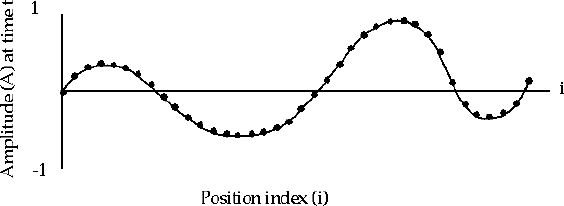
\includegraphics[width=1\textwidth]{pictures/wellengleichung_aufgabe}
	\caption{Schwingung einer Gitarrensaite}
	\label{fig:example_wave}
\end{figure}

Weitere Rahmenbedingungen waren:
\begin{itemize}
	\item Graphical User Interface (Benutzeroberfläche)
	\item Konfiguration per Benutzeroberfläche oder Konfigurationsdatei
	\item Performancevergleich der verschiedenen Varianten
	\item Zwischenpräsentation der Ergebnisse
	\item Paper zum endgültigen Ergebnis
	\item Quellcode-Dokumentation
\end{itemize}

\subsection{Aufbau der Arbeit}
Gegenstand dieser Arbeit sind die Ergebnisse des Projektes und der Weg dorthin. Dies beinhaltet insbesondere den Performancevergleich und die Benutzung der Programme (siehe Rahmenbedingungen).\\
In dieser Arbeit werden zunächst einige Grundlagen zur hier verwendeten Parallelisierung und zu den verwendeten Frameworks erläutert. Des Weiteren gehen wir oberflächlich auf die mathematischen Hintergründe der Aufgabe ein.\\
Anschließend wird die Struktur und der Ablauf unserer drei Programme und wie dieser umgesetzt wurde dargestellt. Schließlich wird gezeigt wie die Anwendungen getestet wurden und zu welchen Schlussfolgerungen wir gekommen sind.